\documentclass[../validierung.tex]{subfiles}
\graphicspath{{./images/}{./1_komponententests/images/}}
\begin{document}

	\section{Einheitstests}
		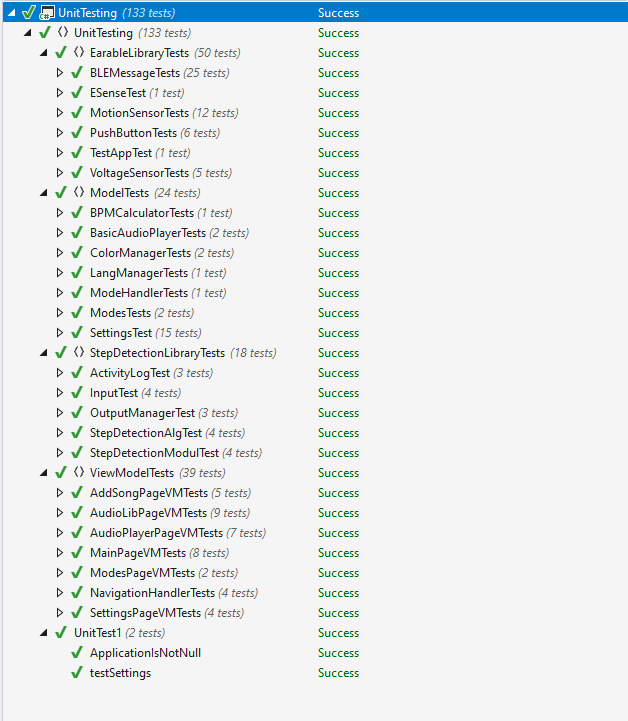
\includegraphics[width=\textwidth]{alleok.png}
		\subsection{Settings Handler Tests}
			\begin{itemize}
				\item\textbf{ColorTest} Testet zurücksetzen der UI Farbe, falls kein Wert in den Properties.
				\item[\textbf{LanguageTest}] Testet zurücksetzten der Sprache, falls Wert unter lang in den Properties ungültig.
				\item[\textbf{LanguageTestNoLangInProperties}]: Testet setzten der Sprache, falls kein Tag lang in den Properties existiert.
				\item UseDifferentLibsTest: Testet das Wechseln zur SpotifyLib \& Ob Playlists \& co. richtig gesetzt werden.
				\item UseDifferentLibsAddThrowsException: Prüft, ob nach dem Wechsel zur SpotifyLib AddTrack eine Exception wirft.
				\item SwitchLibsTest: Wechselt zwischen Spotify{\&}Basic Lib hin und her.
				\item StepsPropertyTest: Testet das Zurücksetzten des Schrittzählers.
				\item ColorPropertyTest: Testet Zurücksetzten \& Setzten der UI Farbe.
				\item SetLangTest: Setzt die Sprache auf eine Test-Sprache.
			\end{itemize}
		\subsection{AudioLib Tests}
			\begin{itemize}
				\item BasicAudioLibAddSongTest: Testet das hinzufügen \& entfernen von mehreren Songs.
				\item BasicLibAddSongNegativeBPMTest: Testet, dass eine ArgumentException geworfen wird, wenn Track mit BMP < 0 hinzugefügt werden soll.
				\item DeleteTrackNonexistant: Testet, dass ArgumentException geworfen wird, wenn nicht existenter Track gelöscht werden soll.
				\item PlaylistBasicLibExceptionTest: Testet, dass Playlist funkitonalität nicht aktiv ist.
				\item SpotifyNonexistantPlaylistTest: Testet, dass ArgumentException geworfen wird, wenn Nichtexistente Playlist gewählt wird.
				\item SpotifyNotImplementedExceptions: Testet, dass mit der SpotifyAudioLib Add \& Delete Track Exceptions werfen.
			\end{itemize}
		\subsection{ModeHandler Tests}
			\begin{itemize}
				\item ResetModeTest: Testet die Reset-Methode des ModeHandler
			\end{itemize}
		\subsection{LangManager Tests}
			\begin{itemize}
				\item ChooseLangTest: Testet das Setzen einer neuen Sprache.
			\end{itemize}
		\subsection{ColorManagerTests}
			\begin{itemize}
				\item ResetColorsTest: Testet, dass nach dem Zurücksetzten der Farben, die Liste der Farben gleich ist.
				\item CurrentColorTest Testet, dass die Current Color anfänglich richtig gesetzt wird.
			\end{itemize}
		\subsection{BasicAudioPlayerTests}
			\begin{itemize}
				\item PlayTrackTest: Tests the PlayTrack Method of the BasicAudioPlayer.
				\item TogglePauseTest: Testet die TogglePause Methode des BasicAudioPlayer.
			\end{itemize}

\end{document}
